\documentclass[12pt]{article}
\usepackage[paperwidth=8.5in,paperheight=11in,margin=1in]{geometry}
\usepackage{float}
\usepackage{lipsum}
\usepackage{parskip}
\usepackage{bbding}
\usepackage{amssymb}
\usepackage{titlesec} 
\usepackage{graphicx}
\usepackage{hyperref}
\usepackage{setspace}
\usepackage[normalem]{ulem}
\usepackage[section]{placeins}
\usepackage[toc,page]{appendix}
\newcounter{subsubsubsection}[subsubsection]
\newcommand{\tline}{\hspace{-2.3pt}$\bullet$ \hspace{5pt}}
\hypersetup{colorlinks=true, linkcolor=black, urlcolor=blue}
\setlength{\parindent}{15pt} % Indent paragraphs (automatically)
\usepackage{pdfpages}

\makeatother
\makeatletter
\setlength{\@fptop}{0pt}

\newcommand\tab[1][1cm]{\hspace*{#1}}

\definecolor{myRed}{RGB}{248, 0, 0}
\definecolor{myGreen}{RGB}{0, 208, 0} %full green isn't dark enough to read
\definecolor{myBlue}{RGB}{0, 0, 248}

\begin{document}
	\begin{titlepage}
		\centering	
%		\vspace{.25cm}
    
    \begin{figure}[h]
      \centering
%      \includegraphics[width=0.45\linewidth]{icon for team goes here}
    \end{figure} 
  
  {\huge\bfseries \textcolor{myRed}{L}\textcolor{myGreen}{E}a\textcolor{myBlue}{D} Design: \\ Team Portfolio\par}
    
    \title{}
    \date{\vspace{-5ex}} %blank date
    \author{%
    	\makebox[.3\linewidth]{\Large\itshape Adrian Beehner}\\Budget Director\\
    	\and \makebox[.3\linewidth]{\Large\itshape Andrew Butler}\\Documenter\\
    	\and \\ \makebox[.3\linewidth]{\Large\itshape Kevin Dorscher}\\Client Liaison\\
    	\and \\ \makebox[.3\linewidth]{\Large\itshape Paul Martin}\\Designer\\
    }
    \let\newpage\relax\maketitle %don't make a new page pls
    \maketitle		
    
    \vspace{4cm} 
    
    {\scshape\Large 
      CS 480/481: Fall 2017 - Spring 2018 \\
      Senior Capstone Design Project \\ 
      UI CS - Wireless Tower of Lights \\
      Sponsor - Dr. Robert Rinker
      \par}
    
     \vspace{4cm} 
    
    \begin{figure}[h]
      \centering
      
\includegraphics[width=0.7\linewidth]{assets/uislogan.png}
    \end{figure} 
  
		\vfill		
	\end{titlepage}

	\tableofcontents
	\newpage
	
	\section{Introduction}
	
		\subsection{Project Summary}
		The University of Idaho has, for several years, done various projects involving the Tower of Lights Show and equipping the marching band with light-up glasses. The current "TowerLights" product involves LED-based light bars that are placed in front of front-facing widows of a large buildling (Theophilus Tower) and are then illuminated to play animations alongside/synchronously with music. The goal is to enhance the current "TowerLights" product. The current implementation of this product uses the ethernet wiring system in the building to control the LEDs. The goal of the project described in this document is to convert this part of the system to a wireless operation. This in turn requires the development of a wireless module that would be attached to each of the light bars. Thus this module has to sleep and wake up, as well as respond to wireless signals from a computer, and since it's wireless, these modules will need to be battery powered. Battery power must also be conserved by staying in the sleep state until needed. The purpose of this enhancement is to provide a certain level of portability to have "TowerLights" at other locations. \\
		The product will give the user the ability to run a program that reads in .tan files and .wav files, have this program communicate with a XBee Wireless module on an Arduino that is attached to a computer via USB, then communicate wirelessly with each Arduino receiver, that is battery powered. Each of these Arduino receivers are attached to an LED board, that will then communicate with each LED on that board through wired communication from the Arduino (same one that holds the receiver) to the LEDs. The program that broadcasts the shows will be available for OSX, Windows, and Linux based operating systems.\\
		This documentation lives at \url{https://github.com/YupHio/LEaD_Design/tree/master/Doc/TeamPortfolio_LEaD_Design.tex} \\
		The code for the project can be found at \url{https://github.com/YupHio/LEaD_Design/tree/master/Code}
		
		\subsection{Document Purpose}
	 		This document is a team portfolio for the Fall 2017-Spring 2018 CS 480/481: Senior Capstone Design project at the University of Idaho. The purpose of this document is to outline the methodology, design, and keep a record of this project. It defines terms used, outlines the scope of the project, details specific design choices, meeting minutes, project learning, design goals, specification and constraints, system diagrams, analysis of alternatives, engineering modeling, manufacturing/assembly plan, experimental design, data analysis, balance sheet, and other items.
		
		\subsection{Definition of Terms}
			\begin{itemize}
				\item \textbf{Arduino} - open source computer hardware and software company, project, and user community that designs and manufactures 		single-board microcontrollers and microcontroller kits for building digital devices and interactive objects that can sense and control objects in the physical world\\ (https://en.wikipedia.org/wiki/Arduino)
				\item \textbf{Arduino Shield} - Shields are boards that can be plugged on top of the Arduino PCB extending its capabilities. The different shields follow the same philosophy as the original toolkit: they are easy to mount, and cheap to produce.\\ (https://www.arduino.cc/en/Main/ArduinoShields)
				\item \textbf{Xbee} - The Arduino Xbee shield allows multiple Arduino boards to communicate wirelessly over distances up to 100 feet (indoors) or 300 feet (outdoors) using the Maxstream Xbee Zigbee module.\\ (https://www.arduino.cc/en/Main/ArduinoShields)		
			\end{itemize}
		
		\subsubsection{Arduino IDE}
		The Arduino Integrated Development Environment - or Arduino Software (IDE) - contains a text editor for writing code, a message area, a text console, a toolbar with buttons for common functions and a series of menus. It connects to the Arduino and Genuino hardware to upload programs and communicate with them. \url{https://www.arduino.cc/en/Main/Software}
		
		\subsubsection{Pulse}
		 PulseAudio is a sound system for POSIX OSes, meaning that it is a proxy for your sound applications. It allows you to do advanced operations on your sound data as it passes between your application and your hardware. Things like transferring the audio to a different machine, changing the sample format or channel count and mixing several sounds into one are easily achieved using a sound server. \url{https://www.freedesktop.org/wiki/Software/PulseAudio/l}
		
	\newpage

\section{Team Meetings and Minutes}
	Weekly action items and summaries of progress made are detailed below. Furthermore, subsections discuss what was helpful and what was not during these meetings. Discussion of attendance and participation, as well as contribution and discussion topics are discussed below.

	\subsection{9/14/2017 Team Meeting 1 Notes}
\noindent
Meeting started at 3:30 in room 133 of the library. Adrian's having Internet issues and is unable to attend. 

\noindent
Project priorities: essentially, everything GUI related should be left until the end. Figuring out, prototyping, and testing hardware is the most important thing this semester.

\noindent
We need to schedule another meeting with Rinker to go over more hardware details. We should create some rough drafts of high level UML diagrams before then, and make sure that we have the big picture correct.

\noindent
What resources (old code, parts, lab space, etc) do we have available right now? 

\noindent
See timeline below

\noindent
Meeting adjourned at 4:16, summary and schedule sent to Adrian afterwards

	\begin{figure}[!htb]
		\centering
		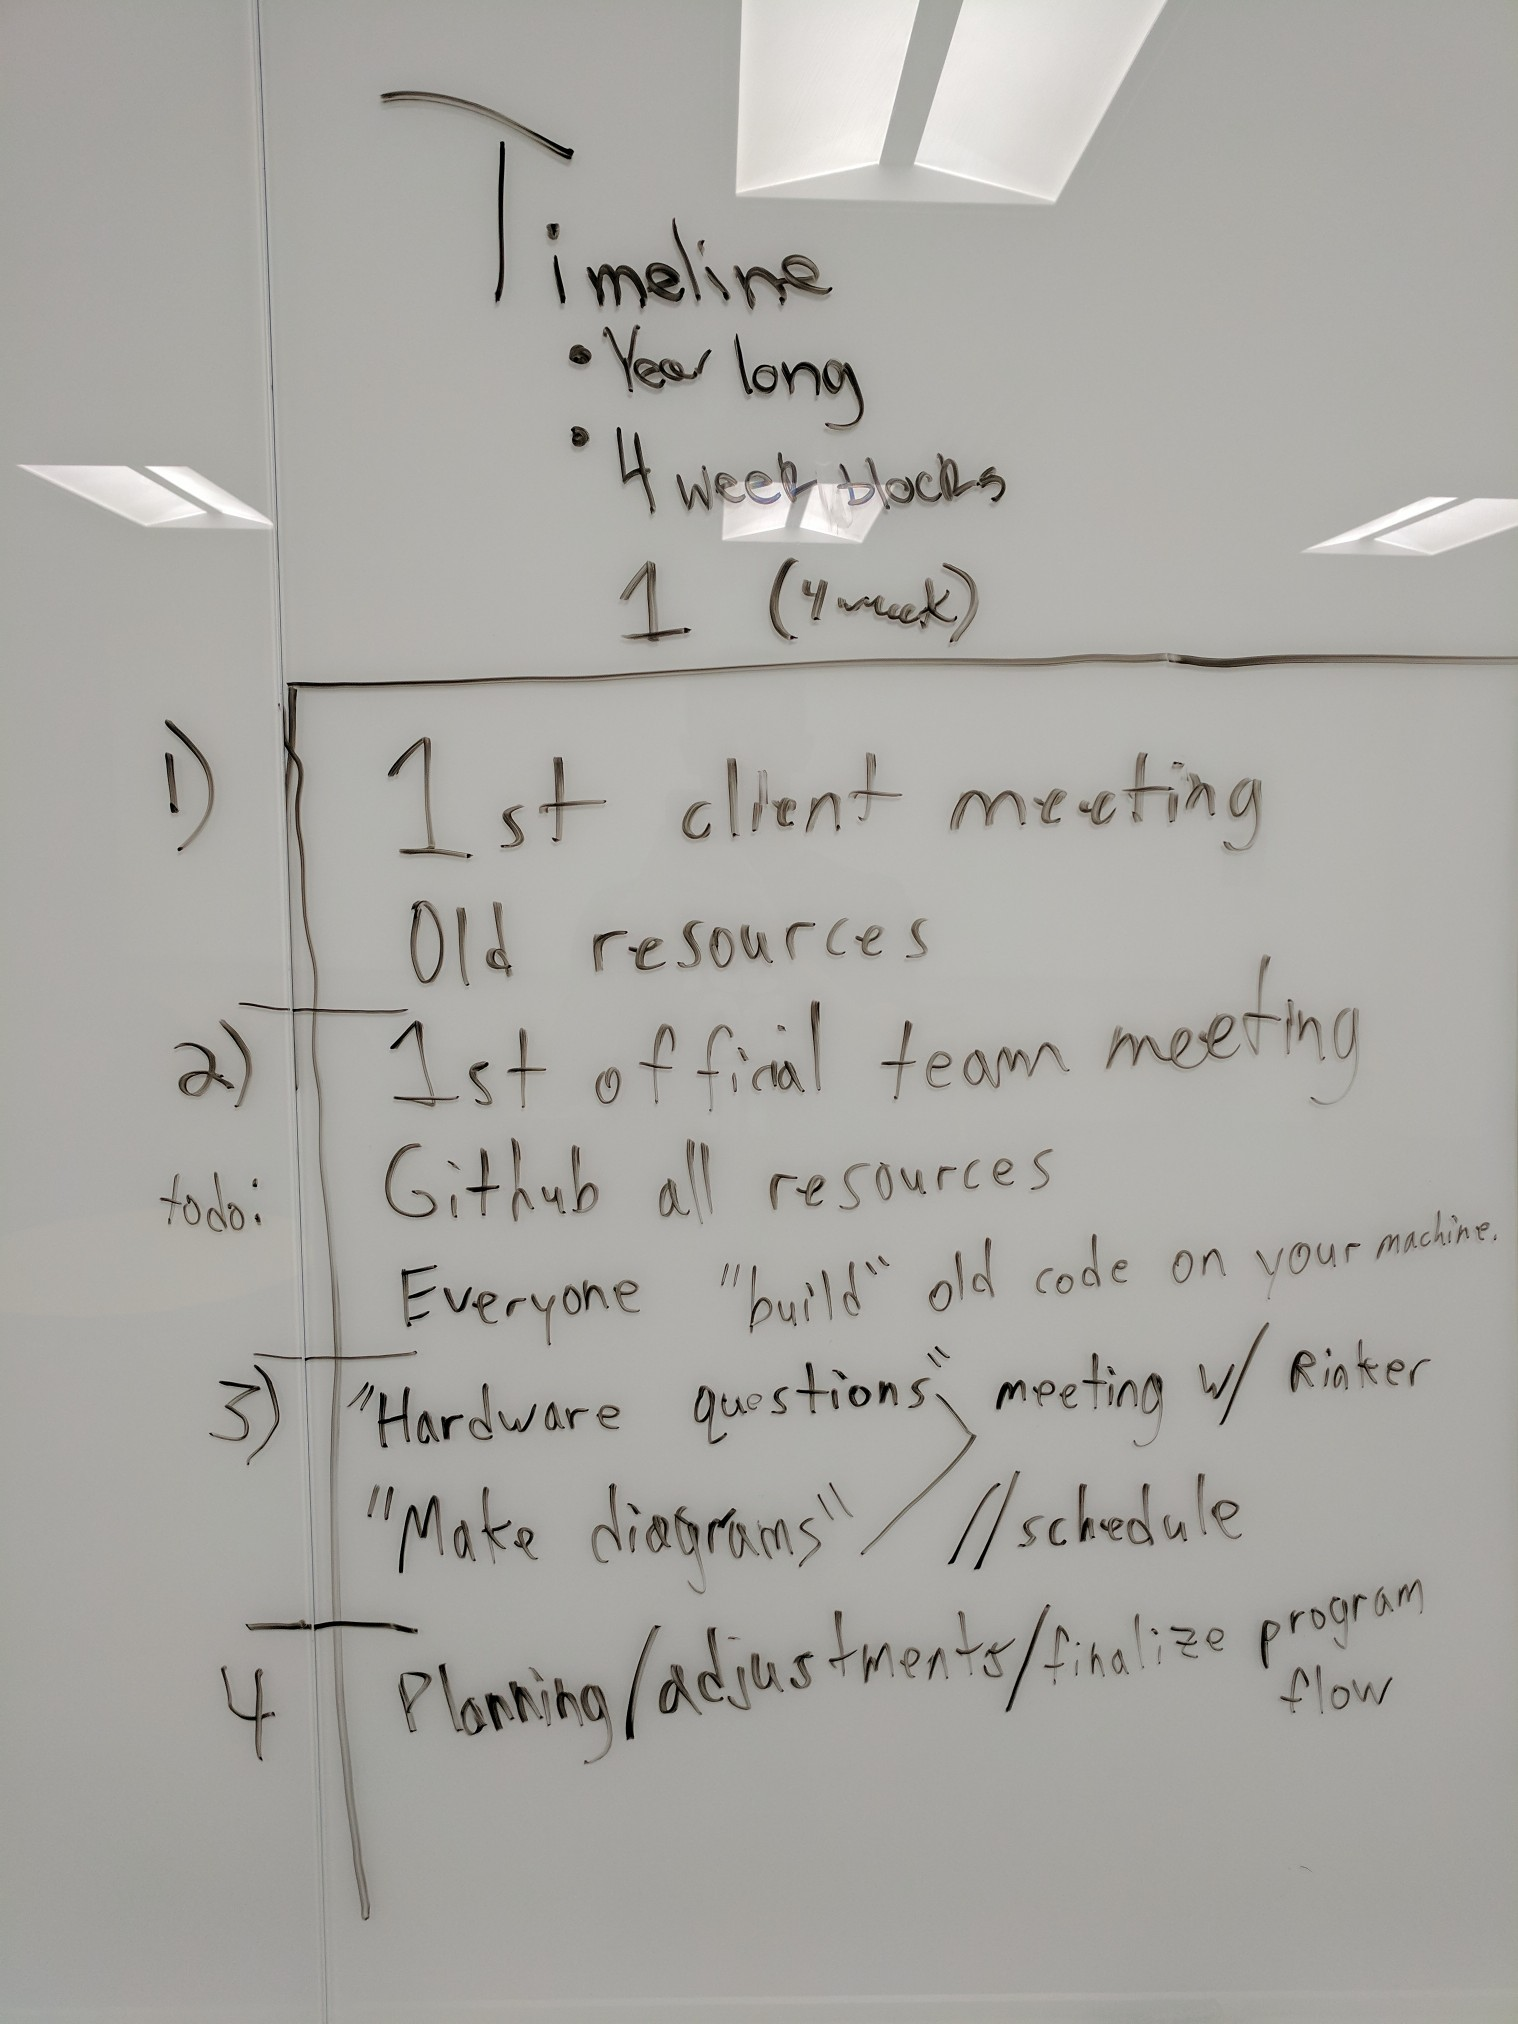
\includegraphics[width=140mm]{assets/9-14_Project_Agenda_1.jpg}
		\caption{9/14 Meeting Project Schedule \label{overflow}}
	\end{figure}

	\begin{figure}[!htb]
		\centering
		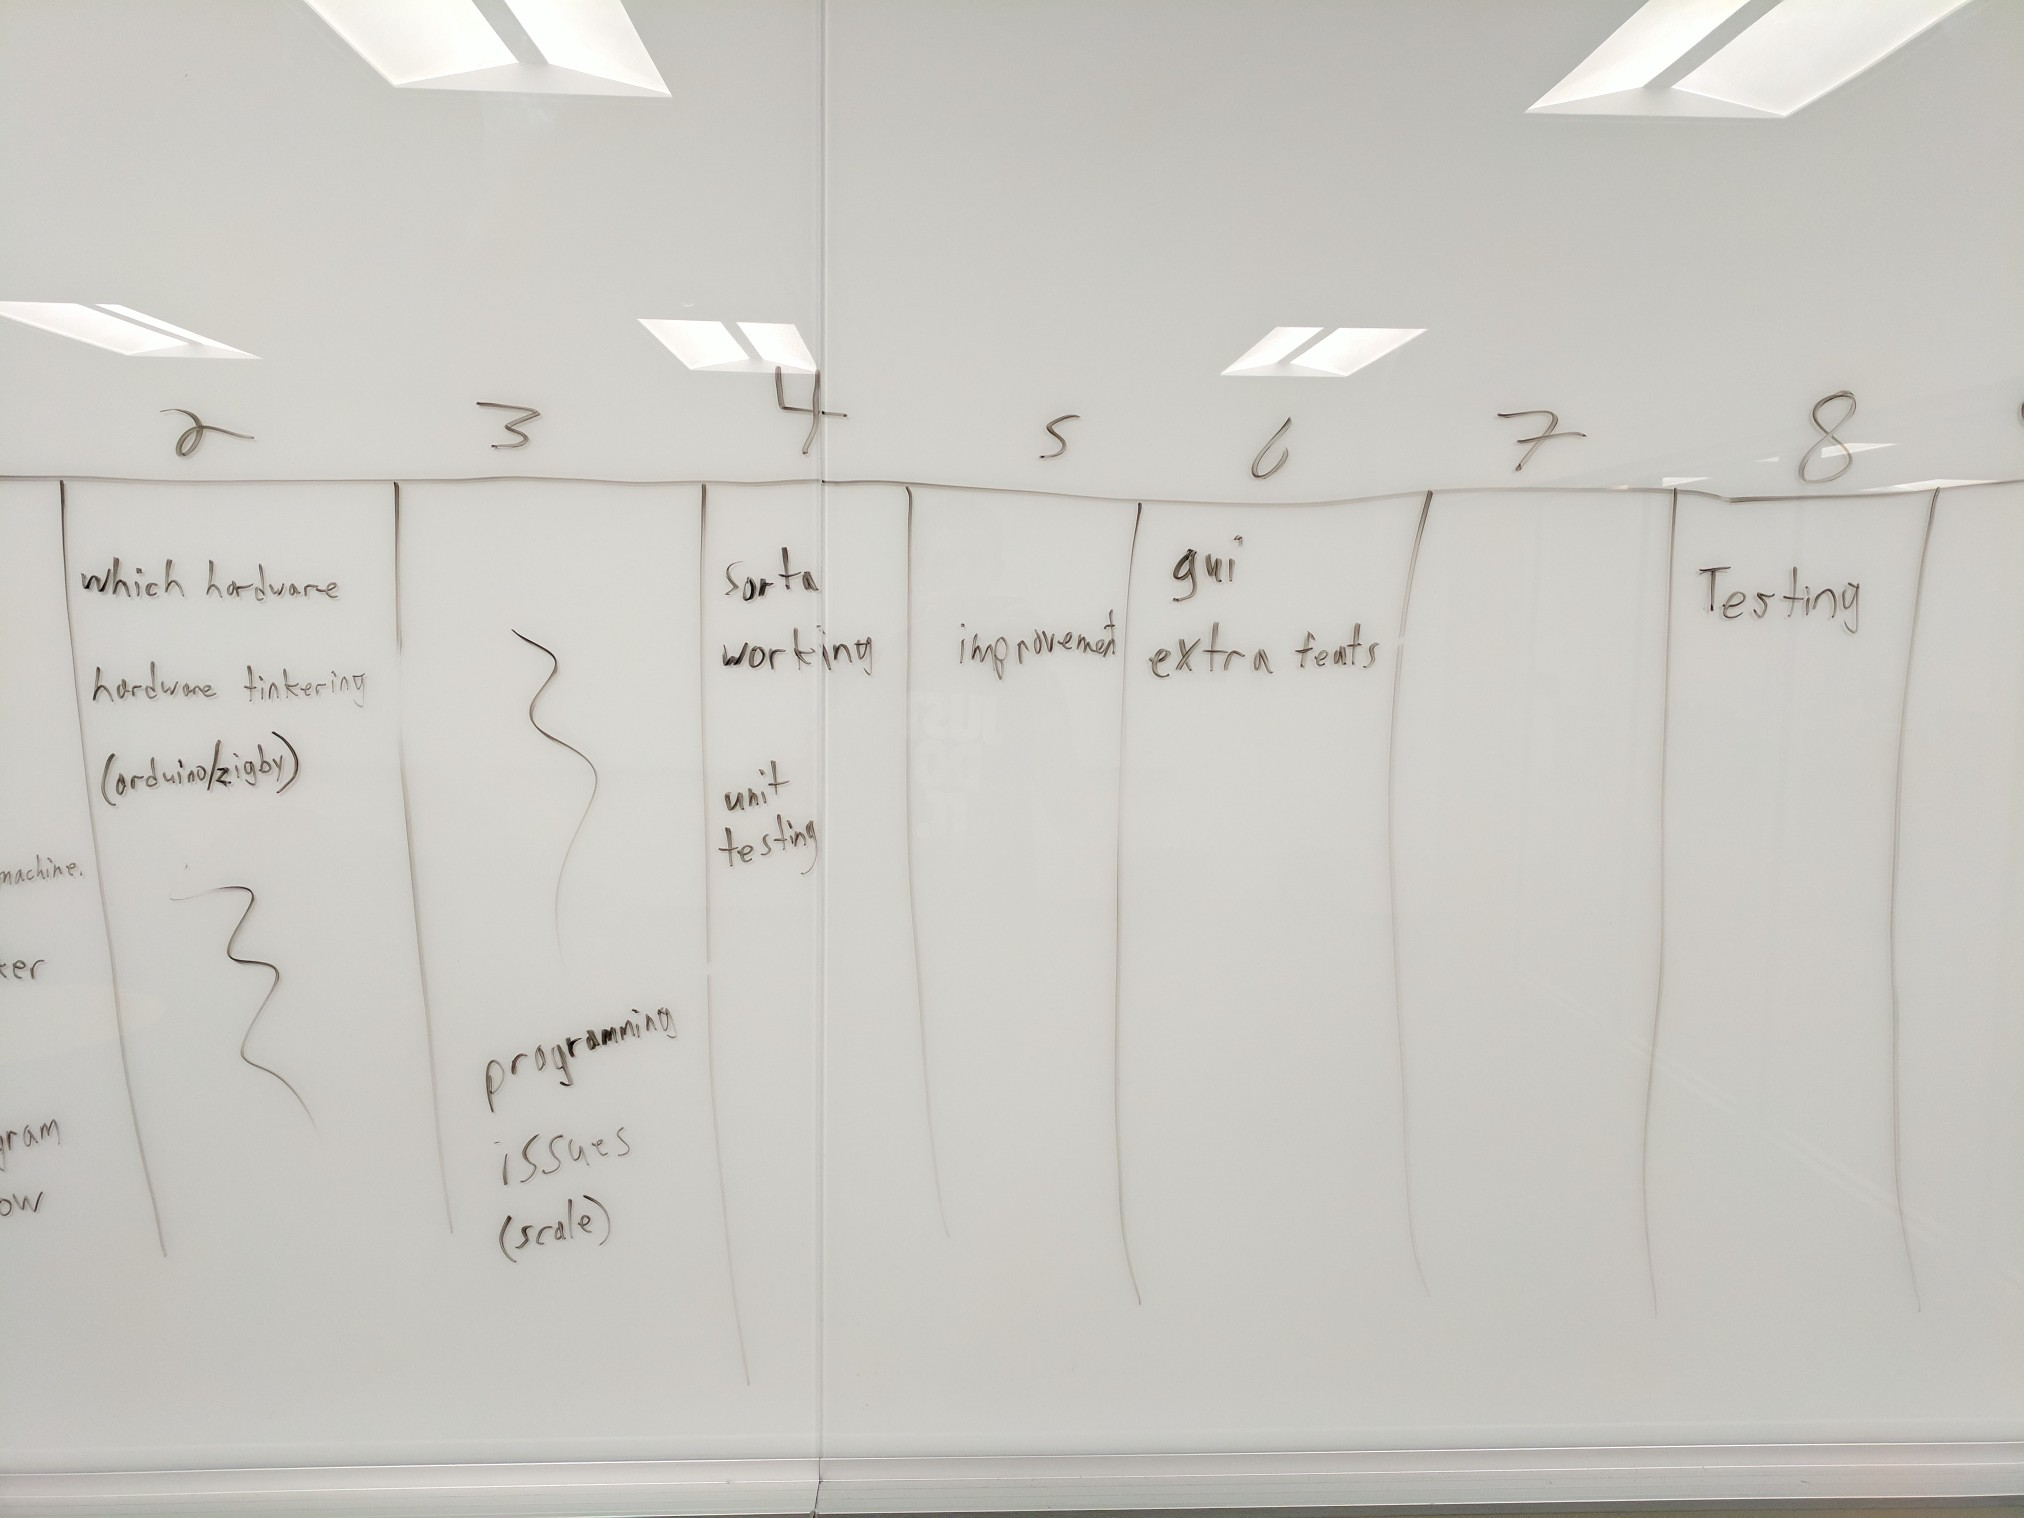
\includegraphics[width=140mm]{assets/9-14_Project_Agenda_2.jpg}
		\caption{9/14 Meeting Project Schedule \label{overflow}}
	\end{figure}
	
	\clearpage

	\subsection{10/05/2017 Team Meeting 2 Notes}

		\noindent
		Meeting started at 3:30, all members except Adrian preset. Adrian’s running a few minutes late due to construction.

		\noindent
		Diagram status and breakdown (Kevin, started 3:31):

		\noindent
		\begin{itemize}
			\item Need to breakdown exactly how the wireless protocol/transmitting will work. Might not be an actual diagram. 
				\begin{itemize}
					\item What frequency?
					\item How many bits/s?
					\item How many bits/packet?
					\item Order/encoding of packets
				\end{itemize}
			\item Breakdown the LEDs
				\begin{itemize}
					\item How many?
					\item Series or parallel?
					\item Total/individual amperage? (~270 mili-amps per currently)
					\item Voltage drop per diode for each color
				\end{itemize}
			\item Battery specifications
				\begin{itemize}
					\item Chemistry/options/alternatives
					\item Voltage
					\item Amp hours/capacity
				\end{itemize}
			\item Receiver/Arduino board
				\begin{itemize}
					\item What code runs on the Atmega328p chips?
					\item LED driver circuit
				\end{itemize}

		\end{itemize}

		\noindent
		Action items (directly off of the diagram status, ~3:48)
		\begin{itemize}
			\item Wireless description (Paul)
			\item LEDs description (Andrew
			\item Battery specification (Adrian)
			\item Receiver/Arduino board specification (Kevin)
		\end{itemize}

		\noindent
		Meeting adjourned at 4:10
	
	\subsection{11/02/2017 Team Meeting 3 Notes}
	Meeting started at 3:29 with all members present, Adrian via Zoom meeting

	\noindent
	Wiki page: Paul’s gotten it started, pages are created and have some content.\\
	
	\noindent
	Meeting tomorrow with Prof. Rinker: allocate a couple hours. The plan is to discuss circuit details, 		assemble hardware to start testing basic functionality.\\ 
	
	\noindent
	Hardware list(Adrian): List has been created, can hopefully be finalized and whatever new parts are 		needed 	to create a prototype can be ordered.\\
	
	\noindent
	Arduino low power mode: 2 interrupt pins, potentially have to be woken up on low level trigger? Look 		more at datasheet and test Arduino this weekend or early next week.\\
	
	\noindent
	Update portfolio: include everything from snapshot day, update timeline, part list/price per unit if we 	can get details from Rinker on time.\\
\begin{itemize}
\item Wireless design spec and wiki page information in portfolio (Paul)
\item Arduino/Receiver design spec and client meeting section in portfolio (Kevin)
\item  Budget decisions, part list, battery specification in portfolio (Adrian)
\item LED design specification, timeline, and team meeting section in portfolio (Andrew)
\item Finish wiki page (Paul)\\
\end{itemize}

Meeting adjourned at 4:10

\clearpage




\section{Client Meetings and Minutes}

	\subsection{9/08/2017 Client Meeting 1 Notes - With Dr.Rinker}

	Meeting started at 3:31, all members present, Adrian on Zoom meeting

Question and Answer with Rinker:

General schedule: Rinker's in CDA start of the week, always in Moscow on Friday, in between depends on events.

Current system in the tower: 3 high powered LEDs (in series) in each room facing the proper direction, controlled over CAT cable from the basement. LEDs prefer constant current over constant voltage, using constant current power source. Each color takes 270 mili-amps. Constant current circuit used here.

Future objectives: Convert system to be wireless. Nodes will need to sleep for a couple days before the show begins, using low power, and should then be remotely wake-able. Power and LED configurations are up to us.

Current goofy lights: broadcast from laptop to Arduino like board, transmits out to the glasses. Wireless protocol related to Zigby. Not wifi, but 802.15.4 (ad-hoc sensor network). Devices can sleep, wakeup, reconnect to network, etc. Zigby handles errors when reconnecting, etc. We avoid using Zigby as we’re broadcasting in real time, and do not want the error handling. Broadcasts on 2.4ghz, regular wifi frequency. 9v lith-ion batteries are being used in the glasses. LEDs in the glasses are in series. Uses a resistor to deliver the correct voltage. Uses the chip from an Arduino, straight up programmed from the Arduino IDE. Atmega328p. Broadcasts to all glasses i.e. DMX. Uses 16 different channels for groups of lights.

802.15.4 only goes at 250kbps. Might want to reduce each channel to 2 bytes instead of 3?

DMX protocol: Used in theater lights, wired protocol, goes through each light sequentially.

Current code is all available for use, we're going to get that from Rinker and put on GitHub(?)

Mouser.com parts. Superbrightleds.com	

Meeting adjourned at 4:39

	\clearpage
	\subsection{9/22/2017 Client Meeting 2 Notes - With Dr.Rinker}
	All members present, Adrian via Zoom, meeting started at 3:32

We only need to deal with .tan file to hardware, there’s another group redesigning the .tan file creator. They’re finishing up in December. Also may be redesigning the interface for the player?

Current implementation uses xbee to transmit to receiver, then transmits to the light controller serially. 

We can probably use old CSAC space to store hardware, work. This has a soldering station too, along with some goofy glasses and the old tower hardware being stored. 

328p chips are super cheap, could definitely use one of those for each light bar. 

Arduino IDE supports turning off bootloader now, etc, which should make development even easier. 

Current player is Linux specific, supposedly has Mac and Windows equivalent libraries though. Pulseaudio and FTDI. Look into making this cross platform compatible.

Main thread of player sends wav bytes to the audio thread, updates lights once the program reaches the proper time. 

Parts needed: transmitter, shield, USB to serial, receiver chips, light bars themselves, batteries. 

Meeting adjourned at 4:33

	\clearpage
	\subsection{11/03/2017 Client Meeting 3 Notes - With Dr.Rinker}
	
	\noindent
	Meeting started at 3:39, all members present, Adrian via Zoom meeting.\\
	
	\noindent
	Constant current circuit: start with the Goofy glasses circuit, figure out what will work for us, 			modify what we need to. Diagrams using PCBArtist(4pcb.com): Each part has a schematic symbol and a 			“footprint” describing what the actual part looks like.\\

	\noindent
	Receiver (MRF chip) can send signals on the 328P’s interrupt pin! Regulator chips should function no 		matter what battery we choose, within reasonable limits, so we should be able to keep using those.\\ 
	
	\noindent	
	Rinker’s going to send us the current circuit diagram so we’ll have access to parts list, details, etc.\\ 
	
	\noindent
	PCBArtist lets you create the traces for the circuit board, then order the custom board based on your 		output. Print as many per sheet as possible, \$33 for each sheet, for students (60 square inches max).\\
	
	\noindent
	Rinker has some breadboard type shields for Arduino that we could use for prototyping if those would be 	helpful. Could basically just add transistors between the Arduino 3.3v supply and the LEDs to create a 		prototype.\\
	 
	\noindent	
	Xbee transmitter is same between Tower Lights and Goofy Glasses.\\ 	

	\clearpage

\section{Project Learning}
	Technologies used to solve problems are described below. Further discussion of these technologies are left in each section's subsections.

	\newpage
  
\section{Design Goals}
	Client needs and project goals are discussed below. A Timeline for these is also included. Discussion of revision of goals, and addition of any new goals is also discussed below.
	
	\subsection{Client Needs}
	The needs of the Client (University of Idaho) are as follows:
		
		\begin{itemize}
			\item LED Light Bars
			\item Microprocessor communication (Arduino)
			\item LEDs bright enough to be a coherent display, visible from a distance in the dark
			\item Wireless Protocol SPI
			\item Battery powered
			\item Receiver Module for Arduino (802.15.14 chip) 
			\item AdrProcessor for designing chip
			\item Low power mode (sleep mode)
			\item Wake up remotely
			\item 1-bit for each color for each window
			\item 802.15.4 protocol, channels 3 bytes (1 for each color, RGB)
			\item Avoid wifi (we don't want to have interference)
			\item Design module
			\item Expand channels (for expanding bandwidth)
			\item 15-20 stories, need to support enough windows
			\item WAV file support
			\item OSX, Windows, and Linux support (Cross-Platform)
			\item .tan file support - 
		\end{itemize}
	
	\subsection{Project Goal}
	The goal of the project is to the extend the versatility of the Tower Of Lights project, which at the moment, gives the user the ability to run a program which reads in a .tan file (animation files for the lights) and .wav files. Then this
	program communicates with a Arduino via Ethernet. Now, the Arduino communicates to each of the LEDs, and tells them which
	color and brightness to be, from the .tan file (thus it basically reads in animation info). 
	The enhancement of the project involves providing cross-platform support, which means having to rework some of the TowerPlayer code so it doesn't use the Pulse library (which is Linux-specific). Also, the enhancement requires making the wired connection to the Arduinos on the LED bar to wireless, this is accomplished by having an Arduino Receiver on each LED Board that receives info sent out from the Arduino connected to the main computer running the program, that Arduino has a XBee Shield attached, which is a wireless module to transmit the info to each Arduino on a board. The Arduino now requires a portable power supply, which needs to be a 9V battery for each Arduino on an LED Board. The final enhancement is that since the LED Boards are running off battery, they require some kind of sleep mode, where they will still be able to receive info (so they can wake up).\\
	
	The product will give the user the ability to run a program that reads in .tan files and .wav files, have this program communicate with a XBee Wireless module on an Arduino that is attached to a Computer via USB, then communicate wirelessly with each battery powered Arduino receiver, on each LED board, that will then communicate with each LED on that board through wired communication from the Arduino (same one that holds the receiver)to the LEDs. The program that runs through this procedure will be available for the OSX, Windows, and Linux based operating systems.

	\subsection{Timeline}
	This is the most recent timeline for the Wireless Tower of Lights project\\
	{ \setstretch{2.0}		
		\scalebox{1}{  		
			\begin{tabular}{r |@{\tline} l}  			
				September  & Planning/Adjustments/Finalize Program Flow         \\			
				October & Hardware Decision/Hardware Tinkering (Arduino/Xbee)            \\			
				November & Hardware Implementation and Initial Prototyping\\			
				December & Prototype Product/Unit Testing     \\			
				January & Product Improvement, Evaluation, and Final Product Hardware Decisions \\			
				February & Implementing and Producing Final Hardware\\			
				March  & Hardware Scale Testing, Software Improvements\\			
				April  & Testing       \\			
				May & Ship/Manufacture (Deliver product)         \\			
			\end{tabular}  		
		}  	
	}
	
	\newpage
    
\section{Specifications and Constraints}
	Discussion of client interviews, pictures, measurements, etc. are provided below. Design specifications and constraints are also presented. Reasoning for any constraints is also mentioned.
	
	\subsection{Arduino / Receiver Design Specification}
	
	\begin{figure}[!htb]
		\centering
		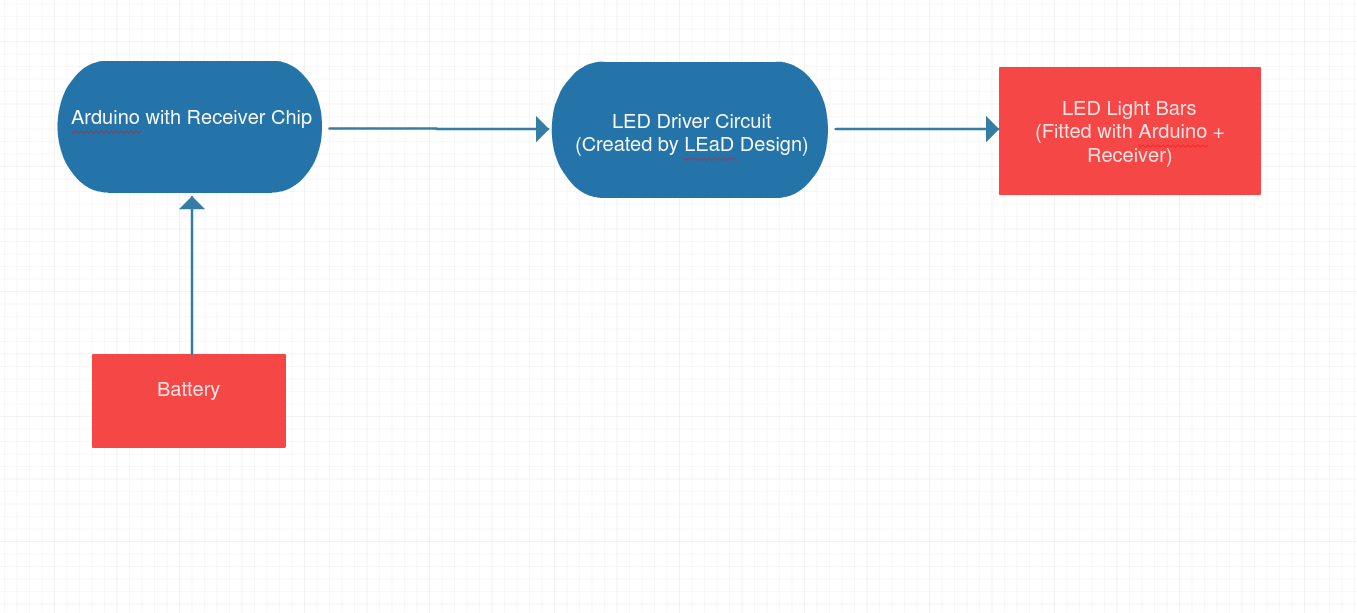
\includegraphics[width = 140mm, height = 95mm]{assets/Arduino_Receiver_Diagram.png}
		\caption{Arduino / Receiver Design Specification \label{overflow}}
	\end{figure}
	
	\indent
	Arduino / Receiver Design Specifications
	\begin{itemize}
		\item Multiple Arduino Atmega 328P boards fitted with a shield and   						  attached receiver chip 
		\item Programming of the individual Arduino Atmega 328P boards using the 					  Arduino IDE (C++)
		\item Receiver chip will delegate the sleep or wake-up modes for each 					  individual light bar
		\item Receiver will also handle input from the transmitting X-Bee, and output 			  data to the LED driver circuit
		\item Creation of the LED Driver circuit which will modify voltage as 						  requested by each set of LED’s to provide a constant current power flow
		\item After modifying voltage accordingly, the LED driver circuit will output 			  the data stream from the receiver to the network that each Arduino 					  Atmega 328P is connected to
	\end{itemize}

	\subsection{Battery Design Specification}
	The list below discusses the attributes for the battery specification, including the requirements, battery chemistry, voltage/capacity, and options/alternatives. Figures "9V Battery Design Specification" and "18650 Lithium Ion Battery Design Specification" corresponding to this information is also shown below.
	
		% Remove Bullets from item list
		{\renewcommand\labelitemi{}
			% Begin list
			\begin{itemize}
				\item \textbf{Requirements}
					\begin{itemize}
						\item Battery required to power the LightBar for TowerOfLights
						\item 3 LEDS on LightBar requires 800 mA
						\item Voltage must be within the range of 8.6 – 9.3 V (Charge)
						\item 10.5 V to run 3 LEDs in a series
						\item 7V for 2 LEDs in a series
						\item Microprocessor based wireless Module distributes the power supply to LEDs on each board
					\end{itemize}
				\item \textbf{Chemistry}
					\begin{itemize}
						\item \textbf{Lithium Ion:} rechargeable battery type, due to high energy density, tiny memory effect, and low self-discharged, lithium ions move from negative electrode during discharge, and back when charging
						\item \textbf{Alkaline:} Popular primary battery (non-rechargeable), dependent on reaction between zinc and manganese dioxide
					\end{itemize}
				\item \textbf{Voltage/Capacity}
					\begin{itemize}
						\item Each LED requires around 3.5 V and each color takes 270 mA
						\item A 9 V battery could support two LEDs in a series, 9V batteries support a wide range of mAh, generally from 400-700 mAh
						\item A 18650 Battery, which has 3.7 V, can be placed in a 18650 holder for 3 batteries, providing 11.1 V, enough to power 3 LEDs in a series (current LightBar setup), with 18650 supporting a range of 1600-3600 mAh
					\end{itemize}
				\item \textbf{Options/Alternatives}
					\begin{itemize}
						\item \textbf{18650 Battery:} large capacity (mAh), allowing LEDs to run longer and can be configured to run LEDs in a series, if making battery pack from these, but requires long charging
						\item \textbf{9V Battery:} Provides smaller capacity, but faster recharge rate. Can only run 2 LEDs for a single 9 V
					\end{itemize}
			\end{itemize}
	
		\begin{figure}[!htb]
			\centering
			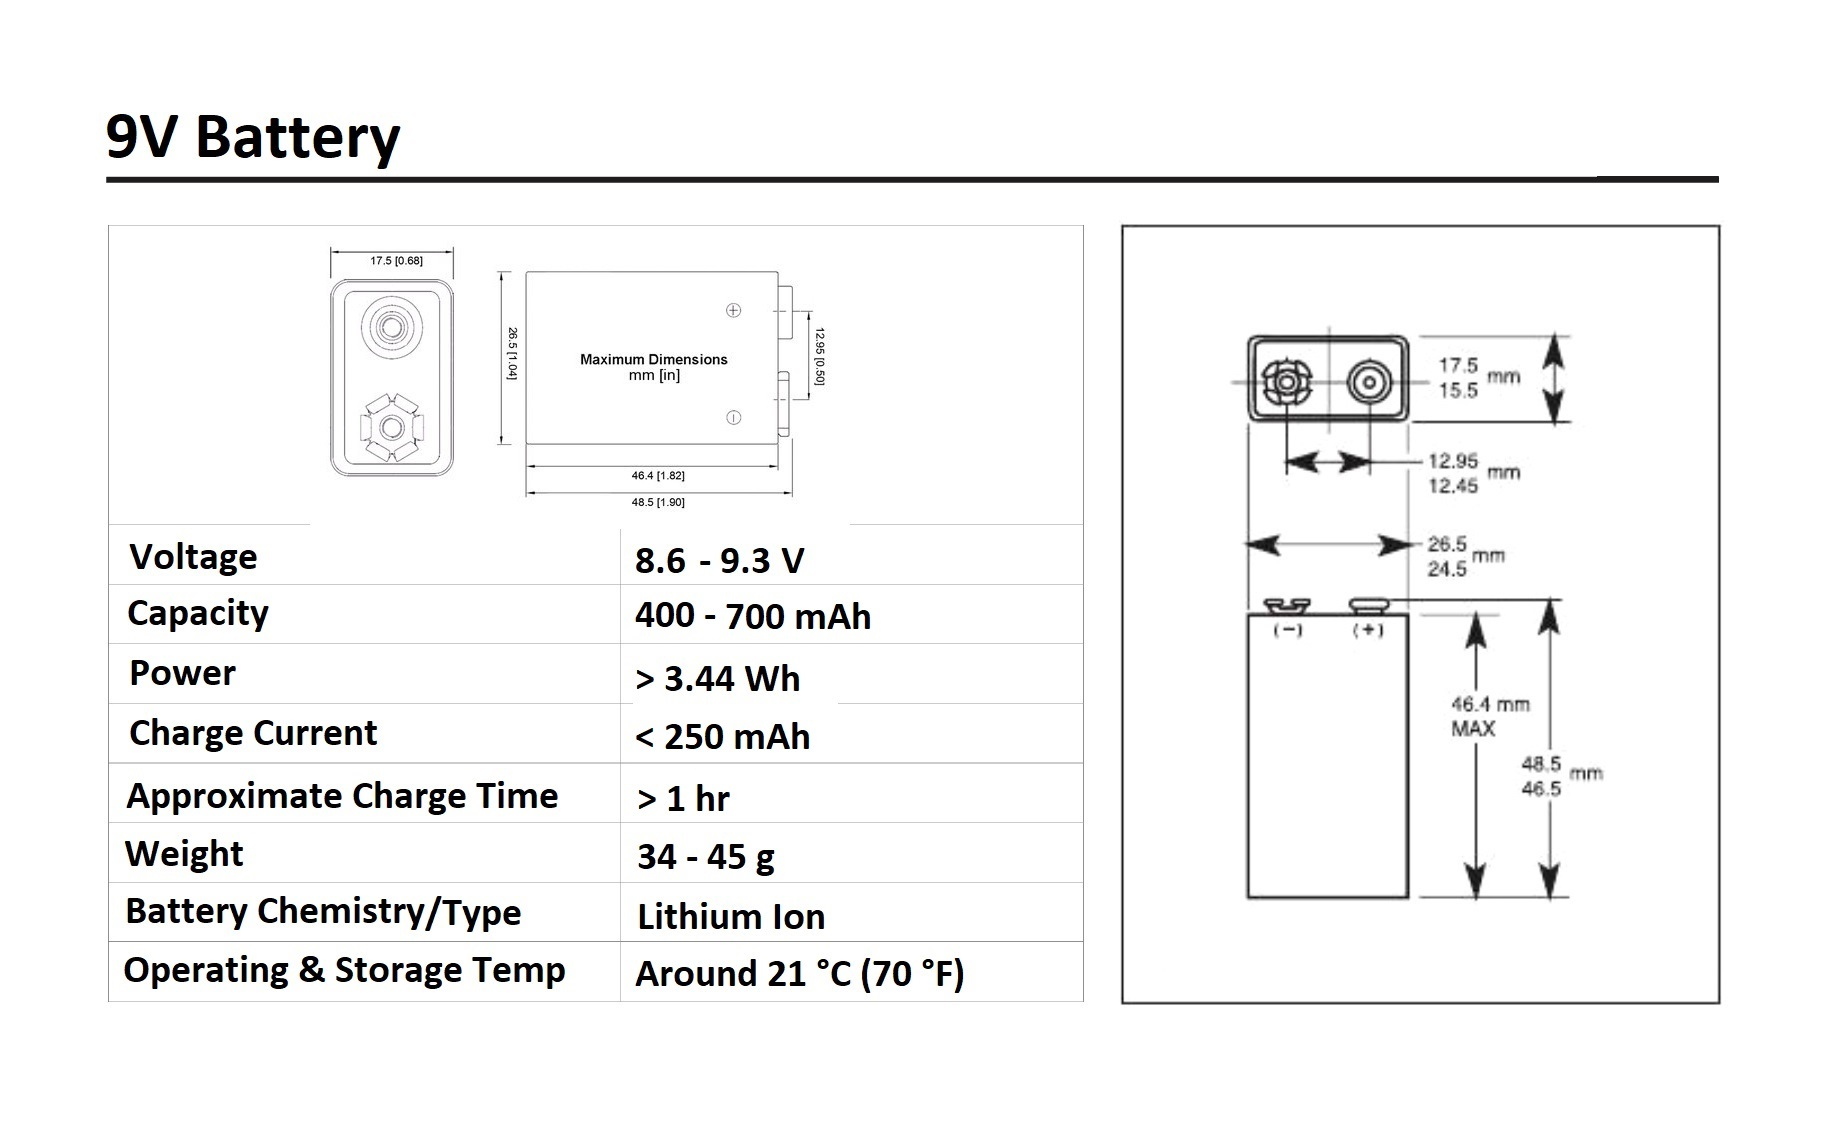
\includegraphics[width = 160mm, height = 100mm]{assets/9V_Battery.jpg}
			\caption{9V Battery Design Specification \label{overflow}}
		\end{figure}
		
		\begin{figure}[!htb]
			\centering
			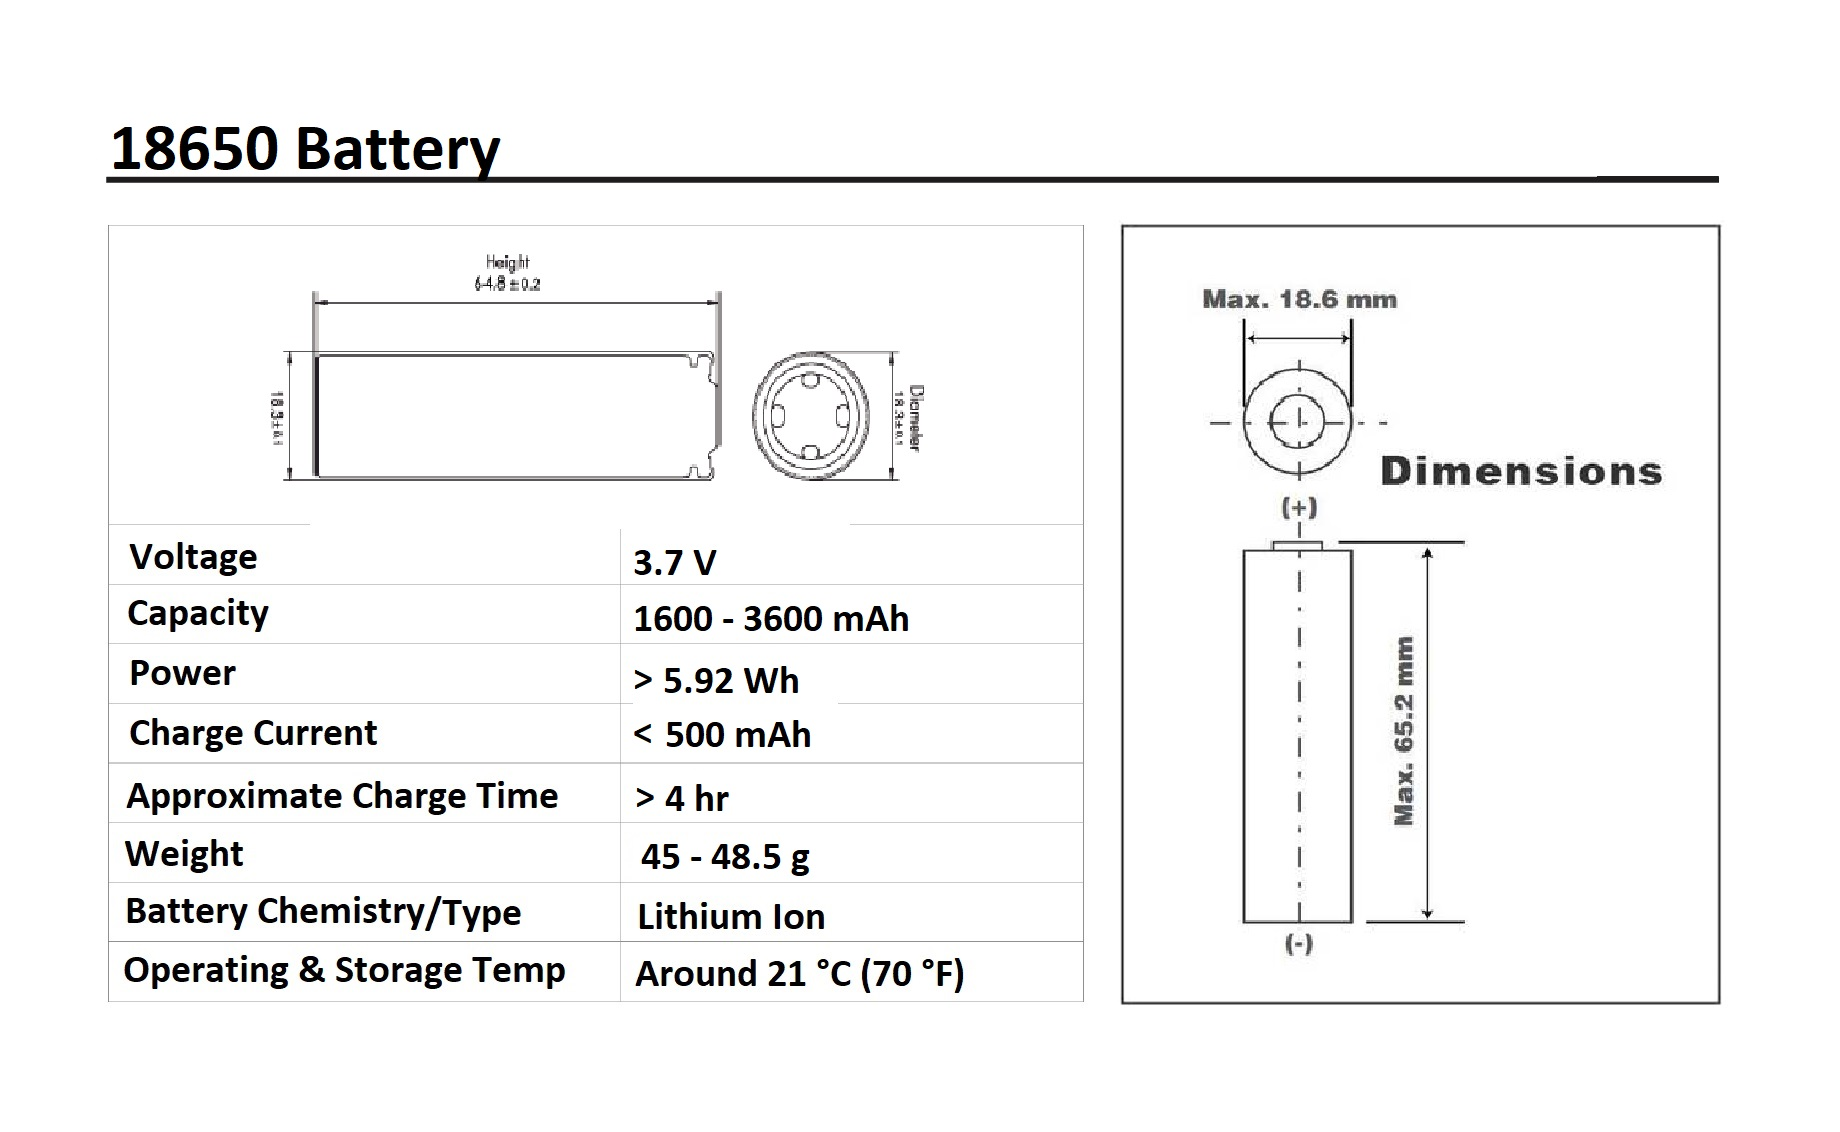
\includegraphics[width = 160mm, height = 100mm]{assets/18650_Battery.jpg}
			\caption{18650 Lithium Ion Battery Design Specification \label{overflow}}
		\end{figure}
		
	% Create new Page (NEED TO USE clearpage because we have pictures that will affect it!)
	\clearpage

	\subsection{LED Design Specification}
	LED specifications and 2 potential solutions detailed below.
	
		% Remove Bullets from item list
		{\renewcommand\labelitemi{}
			% Begin list
			\begin{itemize}
				\item \textbf{Specifications}
					\begin{itemize}
						\item 3 LEDs of each color (red, green, blue) per room
						\item Uses constant current (270-300 mA)
						\item Red LEDs drop ~2.5V per diode
						\item Blue and green LEDs drop ~3.5V per diode
						\item Colors are displayed with pulse-frequency modulation, as each diode can only be fully on or fully off at any moment
					\end{itemize}
				\item \textbf{Circuit Options}
					\begin{itemize}
						\item \textbf{Series:}
							\begin{figure}[!htb]
								\centering
								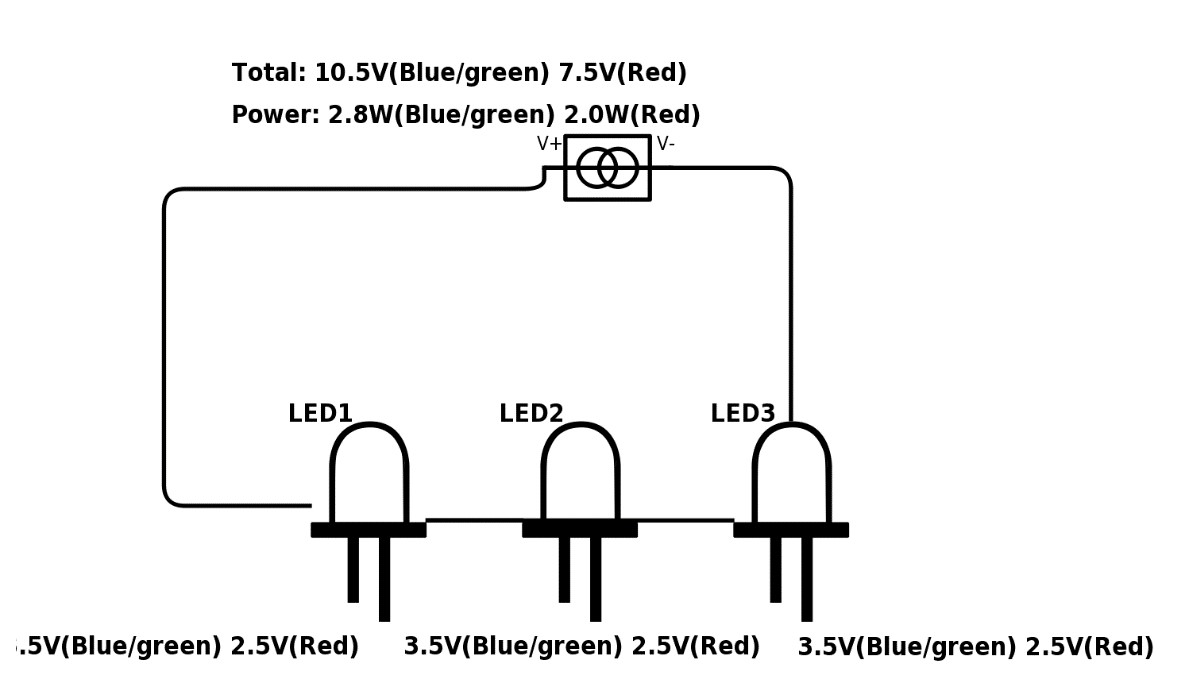
\includegraphics[height = 100mm]{assets/SeriesLED.jpg}
								\caption{Circuit diagram with LEDs in series \label{overflow}}
							\end{figure}
						\item \textbf{Parallel:}
							\begin{figure}[!htb]
								\centering
								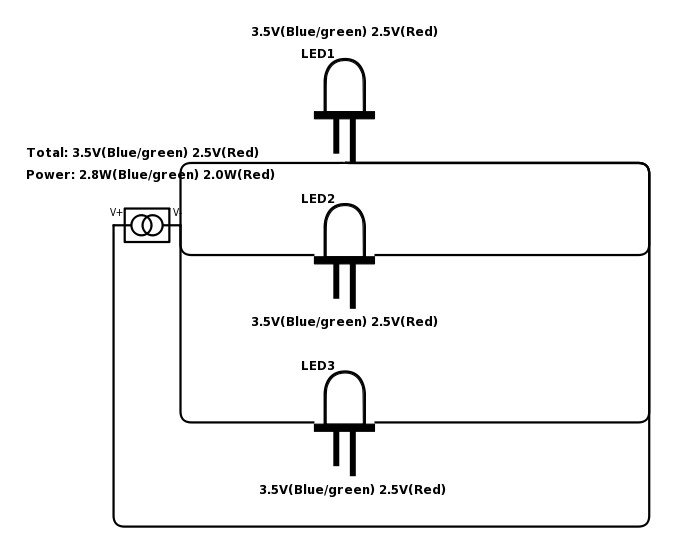
\includegraphics[height = 100mm]{assets/ParallelLED.jpg}
								\caption{Circuit diagram with LEDs in parallel \label{overflow}}
							\end{figure}
					\end{itemize}
			\end{itemize}
	% Create new Page (NEED TO USE clearpage because we have pictures that will affect it!)
	\clearpage
	

\section{System Diagrams}
	Discussion of symbols used, the diagrams themselves, and the software used for the diagrams is discussed below.
	
	\subsection{Current Product}
	The current product flow in regards to the final product is shown below in Figure below. The current setup does not have any battery setup, and requires a wired connection. Changing this is the core of this project, which will improve the versatility of the TowerOfLights product.
	
		\begin{figure}[ht!]
			\centering
			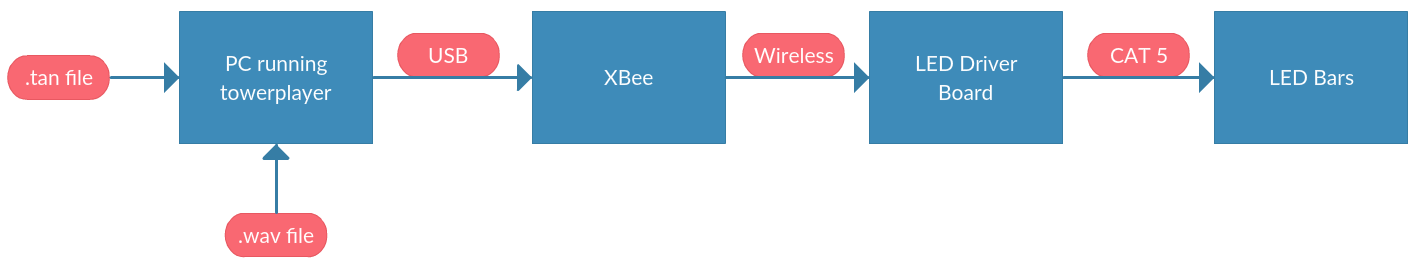
\includegraphics[width=170mm]{assets/What_We_Have.png}
			\caption{Current Product Flow \label{overflow}}
		\end{figure}
	
	
	\subsection{Desired Product}
	The desired product flow is shown in the figure below. The main focus is on the battery that should power each Arduino reciever, as well as the SPI protocol from XBee to the Receiver. This is to make the process wireless instead of wired, which is the main goal of this endeavor.
	
	\begin{figure}[ht!]
		\centering
		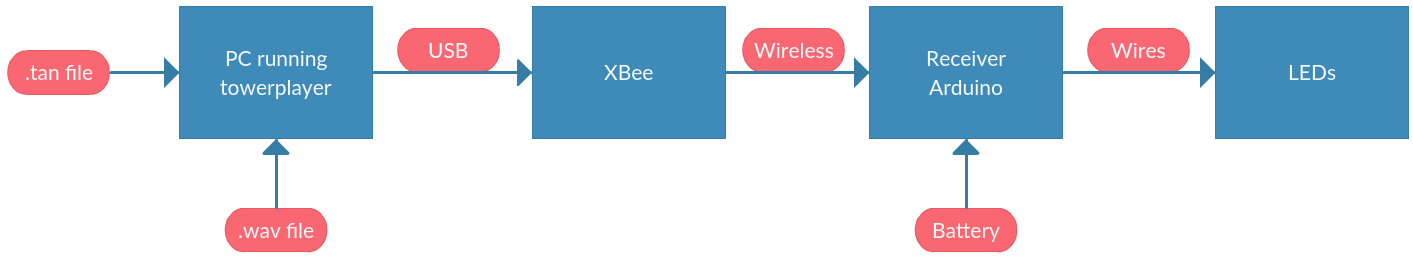
\includegraphics[width=170mm]{assets/What_We_Want.png}
		\caption{Desired Product Flow \label{overflow}}
	\end{figure}


	\subsection{PC Running TowerPlayer}
	The diagram for a flow chart depicting the sequence of actions for running the TowerPlayer program on a computer is shown in the figure below. This diagram helps with understanding the underlying software that needs to be setup and used before the hardware can successfully work together.
	
		\begin{figure}[ht!]
			\centering
			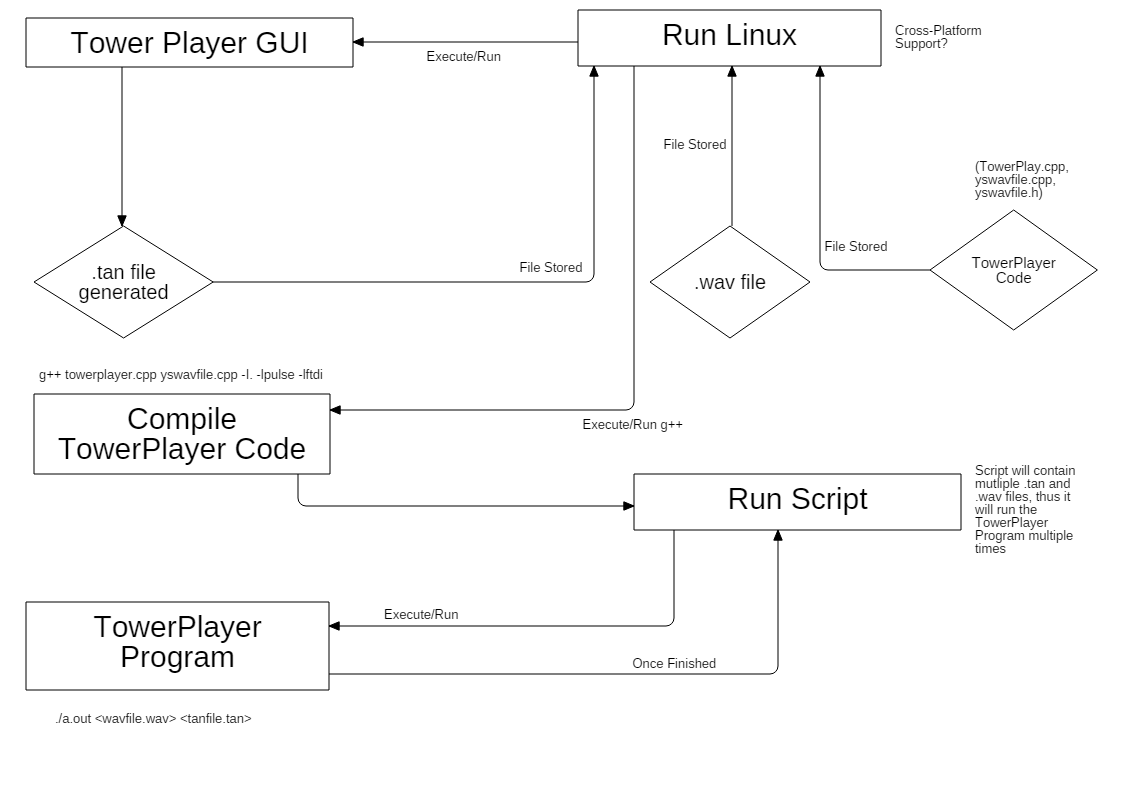
\includegraphics[width=170mm]{assets/PCRunningTowerPlayerFlowChartDiagram.png}
			\caption{Flow Chart Diagram for PC Running TowerPlayer \label{overflow}}
		\end{figure}

	% Create new Page (NEED TO USE clearpage because we have pictures that will affect it!)
	\clearpage

\section{Analysis of Alternatives}
	Discussion of possible alternatives and why some alternatives are better is described below. These topics include: safety, moving parts, cost, durability, compatibility, and reliability.

	\newpage

\section{Engineering Model}
	Discussion of the physical, chemical, and biological system modeling. Also discusses modeling criteria, expected accuracy, and pitfalls. Section of modeling software used is present, as well as data needed and how the data was obtained. Lastly a validation scheme for the model is shown.

	\newpage

\section{Manufacturing/Assembly Plan}
	Discussion of the fabrication need, a flowchart of process oriented projects, a bill of materials, and the estimated manufacturer and delivery time is discussed below.

	\newpage

\section{Experimental Design}
	The characterization of the purpose of the experiment, model validation, data gaps, and performance measurement are discussed below. Also the details on documentation, instrumentation, and measurements are also described.
  	
	\newpage	
  	
\section{Data Analysis}
	Documentation on statistical tools used, accuracy of data, and experiments shown below. Discussion on confidence is results also discussed below.

	\newpage

\section{Balance Sheet}
Discussion on initial budget, estimated cost for materials, components, labor, and spending plan are all described below.

		\subsection{Budget}
		The initial budget of the project itself has yet to be decided. However, the current plan should be to not go over \$500, as the budget/spending of the project should be kept to a minimum. However, as our client's needs are still somewhat 'to be decided' when it comes to how much production of products will be required. In the following subsections, everything will be with the goal in mind to try to keep costs down when ever possible, while still fulfilling client's needs, safety, environmental concerns, and so on. Budgeting is an important factor in this project, since the product is largely hardware-based (while still having some software involved). Evaluating and surveying alternatives and solutions to purchasing and building components is an essential aspect to proper Budgeting for the project.
		
		\subsection{Hardware Decisions}
		Decisions for hardware budget are discussed in the list of topics below, each item discusses the reasons, costs, and possible alternatives that could have been taken when deciding how to properly use the budget.

		% Remove Bullets from item list
		{\renewcommand\labelitemi{}
			% Begin list
			\begin{itemize}
				\item \textbf{Arduino Atmega 328P Chip}
				One of best microcontrollers available, affordable, and works with Arduino boards. Other microcontrollers are the LPXCpresso Boards and ARM Cortex-M4 Microcontroller, these are also affordable micrcontrollers, but they lack the simplicity and versatility that the 328P chips have. 
				\item \textbf{"MuRF" Chip}
				The MRF24J40MA chip is one of the best priced radio transceiver modules, with support for Zigbee protocol, which is the desired protocol for the project, it was the optimal choice. There not really any specific alternatives out there that cater to the needs of the project. Zigbee protocol was the client's desired wireless personal network protocol, and also as benefit to the project, as Zigbee is considered simpler and less expensive than other wireless personal networks such as Bluetooth and Wi-Fi.
				\item \textbf{Xbee Sheild}
				Required Shield/Board to interface with the Program that will transmit the data to the LightBoards. The price of this hardware is somewhat high, due to XBee brand, but since this unit is only required once, for whole product, client will be providing the unit free of charge, this not affecting the budget. Unless the product changed the whole wireless personal network to something other than Zigbee, then this was the only available hardware. 
				\item \textbf{9V Lithium Ion Battery}
				The choice for the 9V Battery was due to the 3 LEDs in a series requiring 10.5V in a series. The only other practical alternative was the 18650 lithium battery. However when it comes down to size, mAh, and Voltage, the 18650 battery is the better option, however price is also a large factor, and the 9V wins there.
				\item \textbf{18650 Lithium Ion Battery}
				The choice for the 18650 Battery was due to the 3 LEDs in a series requiring 10.5V in a series. The only other practical alternative was the 9V lithium battery. However when it comes down to size, mAh, and Voltage, the 18650 battery is the better option, however price is also a large factor, and the 9V wins there.
				\item \textbf{Common Anode RGB LED}
				This was a fairly simple choice, as there really is only one type of LED that will work properly for the project, as the product requires the standard LEDs with three dinodes for each color, 3.5V for Red and Green, and 2.5V for Red.
				\item \textbf{LightBar Board}
				This was requested by the client, needed a board to house the product, this is fairly cheap, as it it just na board to house the hardware for the product. The materials/quality of materials to build the board at least at the moment are TBD, while a simple wood board will probably suffice. The size of the board is required to be 1 in x 2 in, thus with this estimate the board would be a fair price for housing the hardware, and providing easy assembly (since with wood the parts can be screwed in).	
				\item \textbf{LED Driver Circuit}
				The actual LED Driver Circuit will be designed by the team, thus there won't be an additional cost in designing, as once the design is done, there are companies that allow the consumer to design PCBs (Printed Circuit Boards) and then order as many PCBs as needed. The company that LEaD Design will be working with to order the circuits is 4PCB, a company that "Specializes in printed circuit board manufacturing and PCB assembly, including prototype and production circuit boards" (www.4pcb.com). They offer special discounts to students, where a 60 $in^2$ board can be created for \$33, and the consumer can put any amount of PCBs, as long as they fit within the 60 $in^2$ size (the 60 $in^2$ is not limited to 6 in x 10 in either, it can be any dimension that fits 60 $in^2$). Thus until the design of the LED Driver Circuit is done, the actual cost per unit of it cannot be determined. The goal in the design process will be to try to make the circuit as small as possible while fulfilling the requirements and keeping in mind the manufacturing process of the circuit (if it is too small, it will be difficult to attach the circuit to rest of the product).
			\end{itemize}
			
			\subsection{Hardware List/Cost of Materials}
			The figure below is the current Hardware list, describing the physical components of the product, their required quantity, and cost per unit. These specifications are still subject to change and evaluation.
			
			\begin{figure}[ht!]
				\centering
				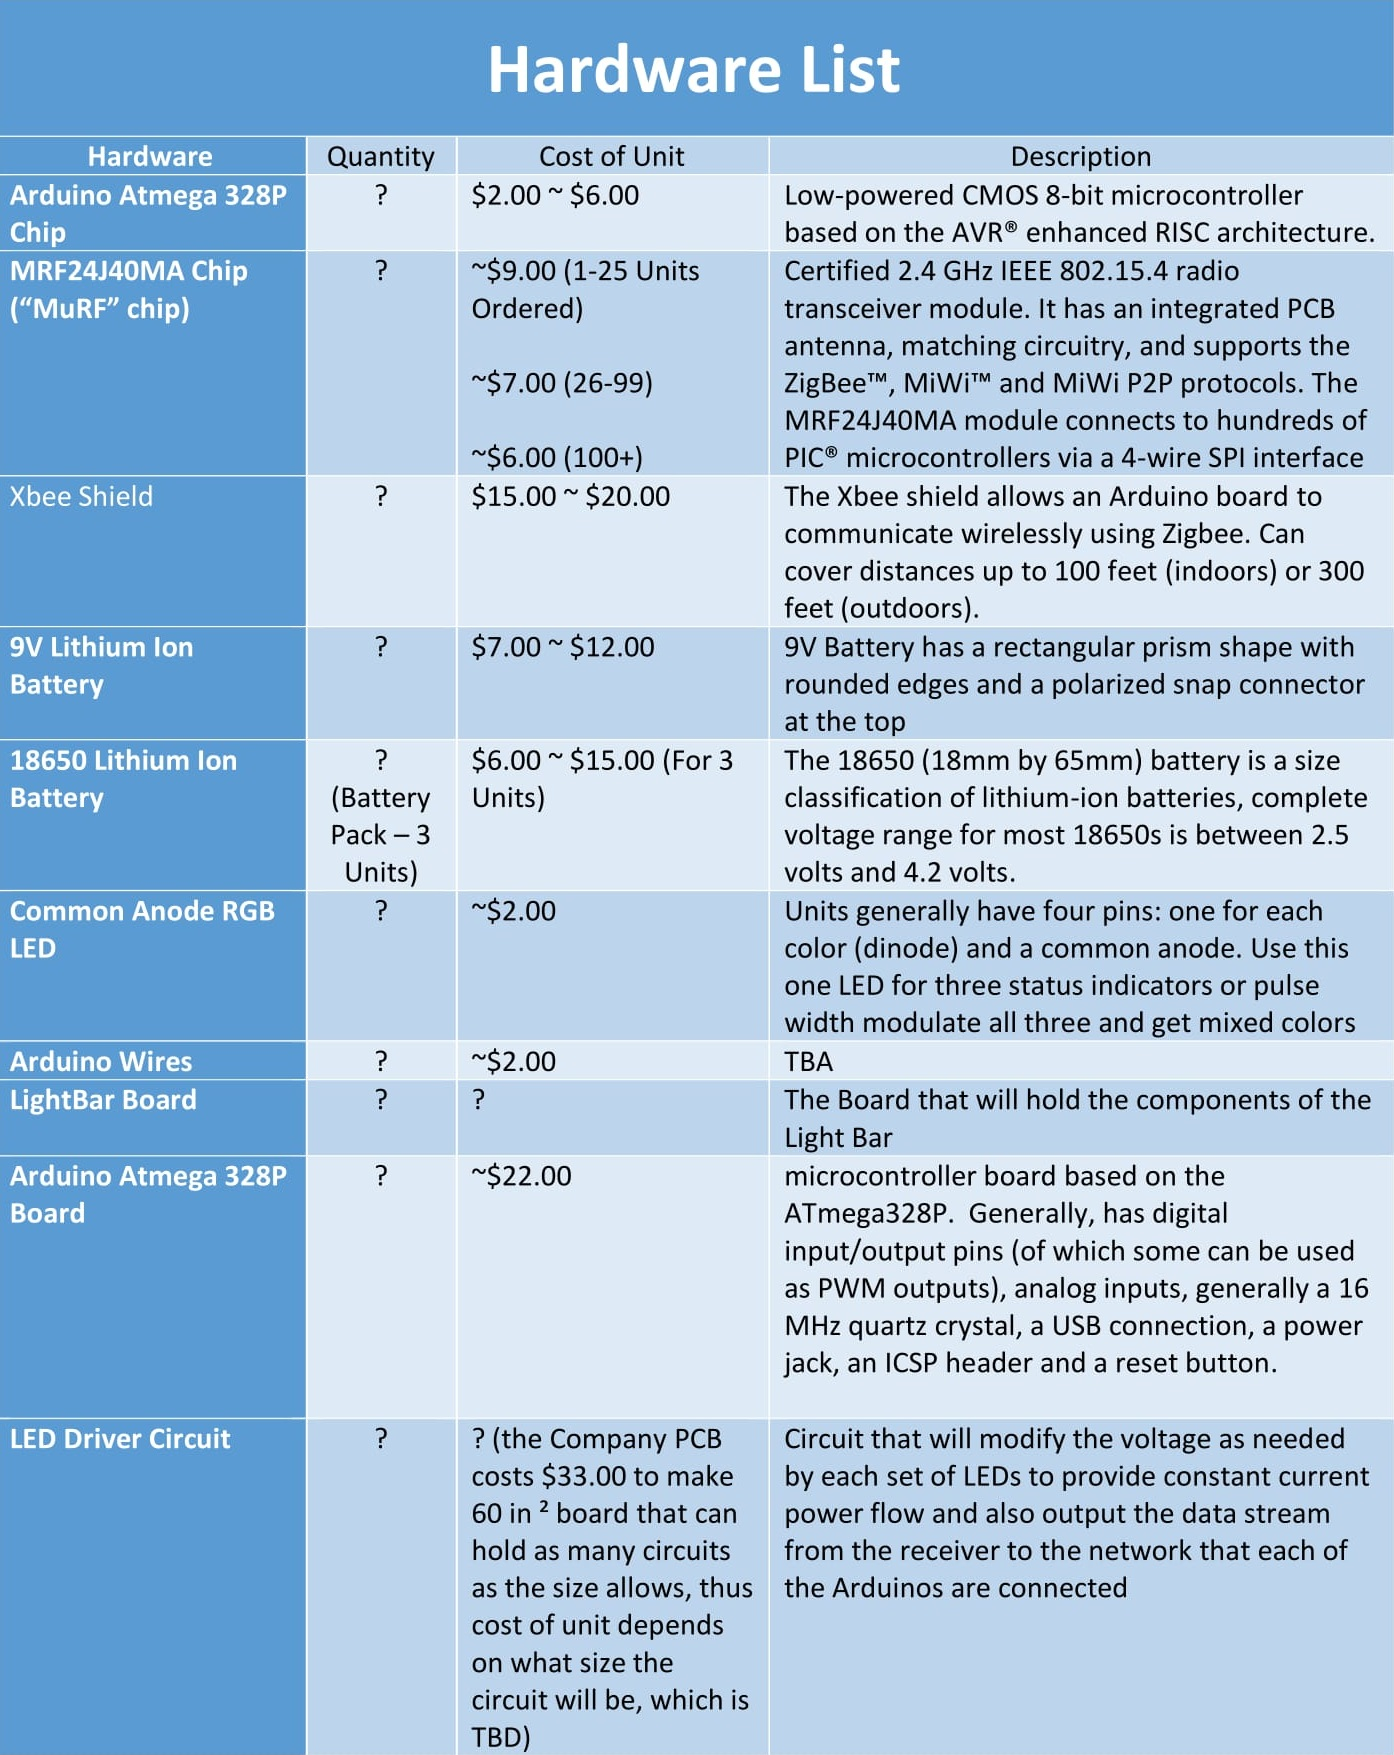
\includegraphics[width=170mm]{assets/HardwareList.jpg}
				\caption{Hardware List \label{overflow}}
			\end{figure}
			
			\newpage

\section{Other Items}
	File management, archiving, documenting any issues, reports of accidents/incidents/near misses/precautions are described below. 
	
	\subsection{LEaD Design Team Contract}
	The team contract for the \textit{LEaD Design} is shown below. The contract discusses the various professional approaches the team will be held accountable to act towards during the time spent on the project. The contract is an important document, as it dicusses the various inner workings of how the team will work on assignments, resolve conflicts, manage work, make decisions and so on. The contract is four pages total.
	
		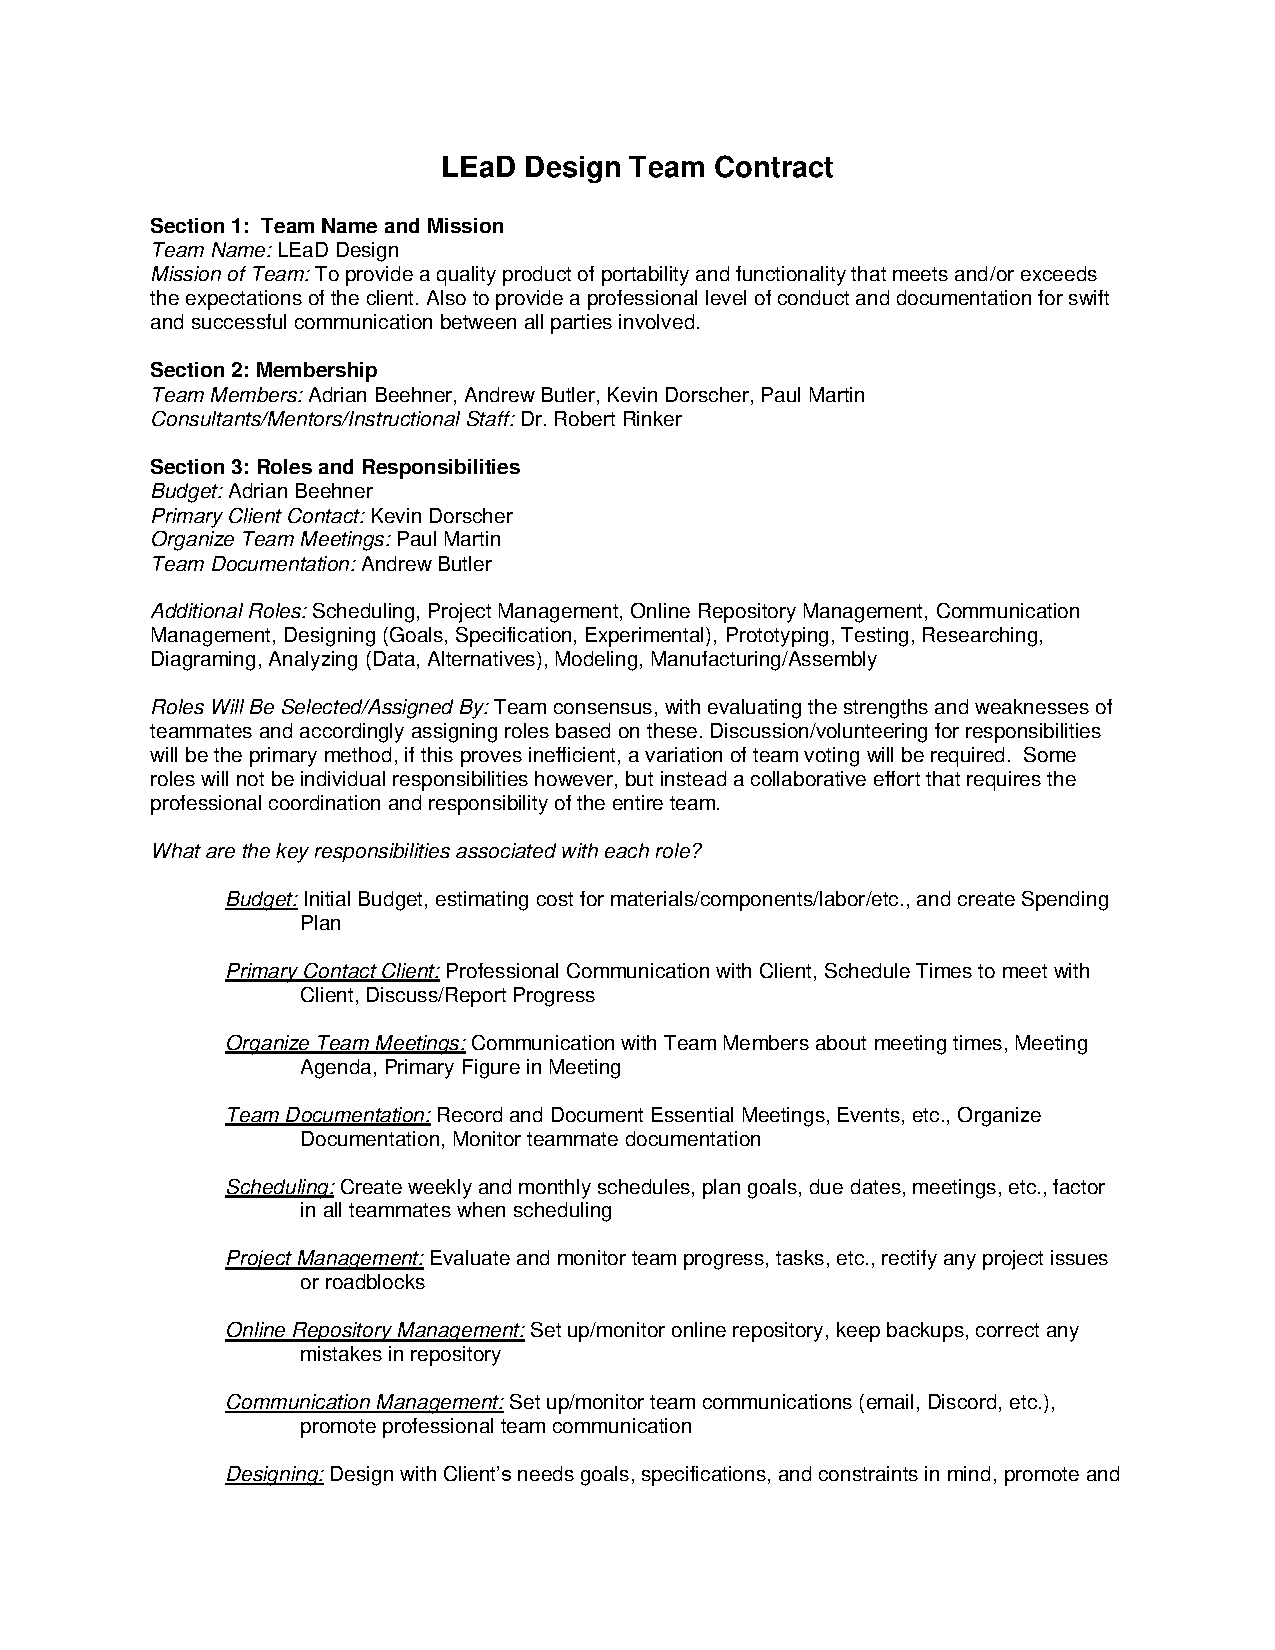
\includepdf[pages={-}, scale =1, pagecommand={}]{assets/LEaD_Design_Team_Contract.pdf}			% {-} means include all pages
		


\end{document}
